\documentclass[border=2mm,12pt]{standalone}
\usepackage{tikz}

\begin{document}
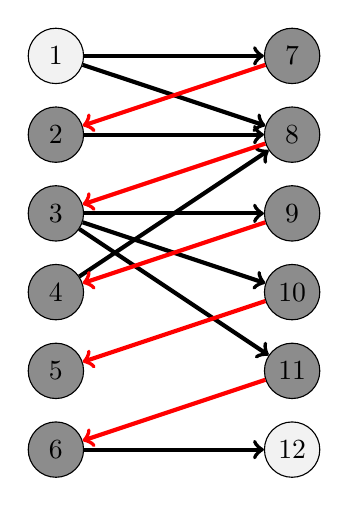
\begin{tikzpicture}[
    xscale=1.5, 
    every node/.style={draw, circle, minimum size=20pt, inner sep=-5pt}
]

    \node[fill=gray!10] (1)  at (-1, -1) {1};
    \node[fill=gray!90] (2)  at (-1, -2) {2};
    \node[fill=gray!90] (3)  at (-1, -3) {3};
    \node[fill=gray!90] (4)  at (-1, -4) {4};
    \node[fill=gray!90] (5)  at (-1, -5) {5};
    \node[fill=gray!90] (6)  at (-1, -6) {6};
    \node[fill=gray!90] (7)  at (1, -1)  {7};
    \node[fill=gray!90] (8)  at (1, -2)  {8};
    \node[fill=gray!90] (9)  at (1, -3)  {9};
    \node[fill=gray!90] (10) at (1, -4)  {10};
    \node[fill=gray!90] (11) at (1, -5)  {11};
    \node[fill=gray!10] (12) at (1, -6)  {12};

    \draw[->,line width=1.5pt] (1) -- (7);
    \draw[->,line width=1.5pt] (1) -- (8);
    \draw[->,line width=1.5pt] (2) -- (8);
    \draw[->,line width=1.5pt] (3) -- (9);
    \draw[->,line width=1.5pt] (3) -- (10);
    \draw[->,line width=1.5pt] (3) -- (11);
    \draw[->,line width=1.5pt] (4) -- (8);
    \draw[->,line width=1.5pt] (6) -- (12);

    \draw[->,line width=1.5pt, color=red] (7) -- (2);
    \draw[->,line width=1.5pt, color=red] (8) -- (3);
    \draw[->,line width=1.5pt, color=red] (9) -- (4);
    \draw[->,line width=1.5pt, color=red] (10) -- (5);
    \draw[->,line width=1.5pt, color=red] (11) -- (6);

\end{tikzpicture}
\end{document}
